\documentclass[11pt]{article}

\usepackage[margin=1in]{geometry}
\usepackage[T1]{fontenc}
\usepackage{lmodern}
\usepackage{microtype}
\usepackage{amsmath}
\usepackage{graphicx}
\usepackage{float}
\usepackage{booktabs}
\usepackage{xcolor}
\usepackage{caption}
\usepackage{titlesec}
\usepackage[hidelinks]{hyperref}
\usepackage{color,soul}

\definecolor{accentcol}{HTML}{1B5E73}
\titleformat{\section}{\normalfont\large\bfseries\color{accentcol}}{\thesection.}{0.6em}{}
\titleformat{\subsection}{\normalfont\normalsize\bfseries}{\thesubsection}{0.6em}{}
\titlespacing*{\section}{0pt}{14pt}{6pt}
\titlespacing*{\subsection}{0pt}{10pt}{4pt}
\captionsetup{font=small,labelfont=bf,labelsep=period}

\newcommand{\dpr}{d^{\prime}}

\hypersetup{pdftitle={BODMAS: Combined Results}}

\begin{document}

\begin{center}
{\LARGE\bfseries Results}\\[6pt]
{\large Detecting Order-of-Operations Misconceptions from a Student's Written Work:\\[2pt]
Humans, a Bayesian Ideal Observer, and LLMs on the Same 240-Item Pool}\\[10pt]
{\small Draft compiled \today}
\end{center}

\section{Bayesian ideal observer: one-misconception items}\label{sec:bayes-1misc}

The ideal observer inverts the generative learner model: given a trace, it computes a
posterior over all 22 learner profiles (the expert, 6 single misconceptions, 15 pairs) and
reports the marginal probability that the misconception \emph{named in the belief statement}
is part of the student's policy, $P(\text{named rule} \mid \text{trace})$. This marginal is
its analog of the human 1--6 agreement rating; 0.5 is the neutral point. The one-misconception
items are the 120 items of categories A and B: in A the statement names the misconception that
generated the work (agreeing is correct), in B it names one that is absent (disagreeing is
correct). Each misconception contributes exactly 10 items to each category.

\subsection{Category A: the named misconception is present}\label{sec:bayes-1misc-a}

Figure~\ref{fig:bayes1a} shows the distribution of the per-item marginal, one panel per
misconception present in the trace (in category A the present and named misconceptions
coincide by design, so no other grouping exists). All of the probability mass sits at the far
right of the scale: every one of the 60 items lands between 0.82 and 1.00, far above the 0.5
decision point, so thresholded accuracy is 100\% for every misconception. Five of the six
misconceptions concentrate in a narrow 0.92 to 1.00 band. \sethlcolor{green} \hl{The exception is \texttt{outside\_bracket\_first}, whose whole distribution is shifted left (0.82 to 0.93):
bracket evidence is systematically the weakest of the six, a property of most of its items
rather than of a few outliers.}

\begin{figure}[H]
\centering
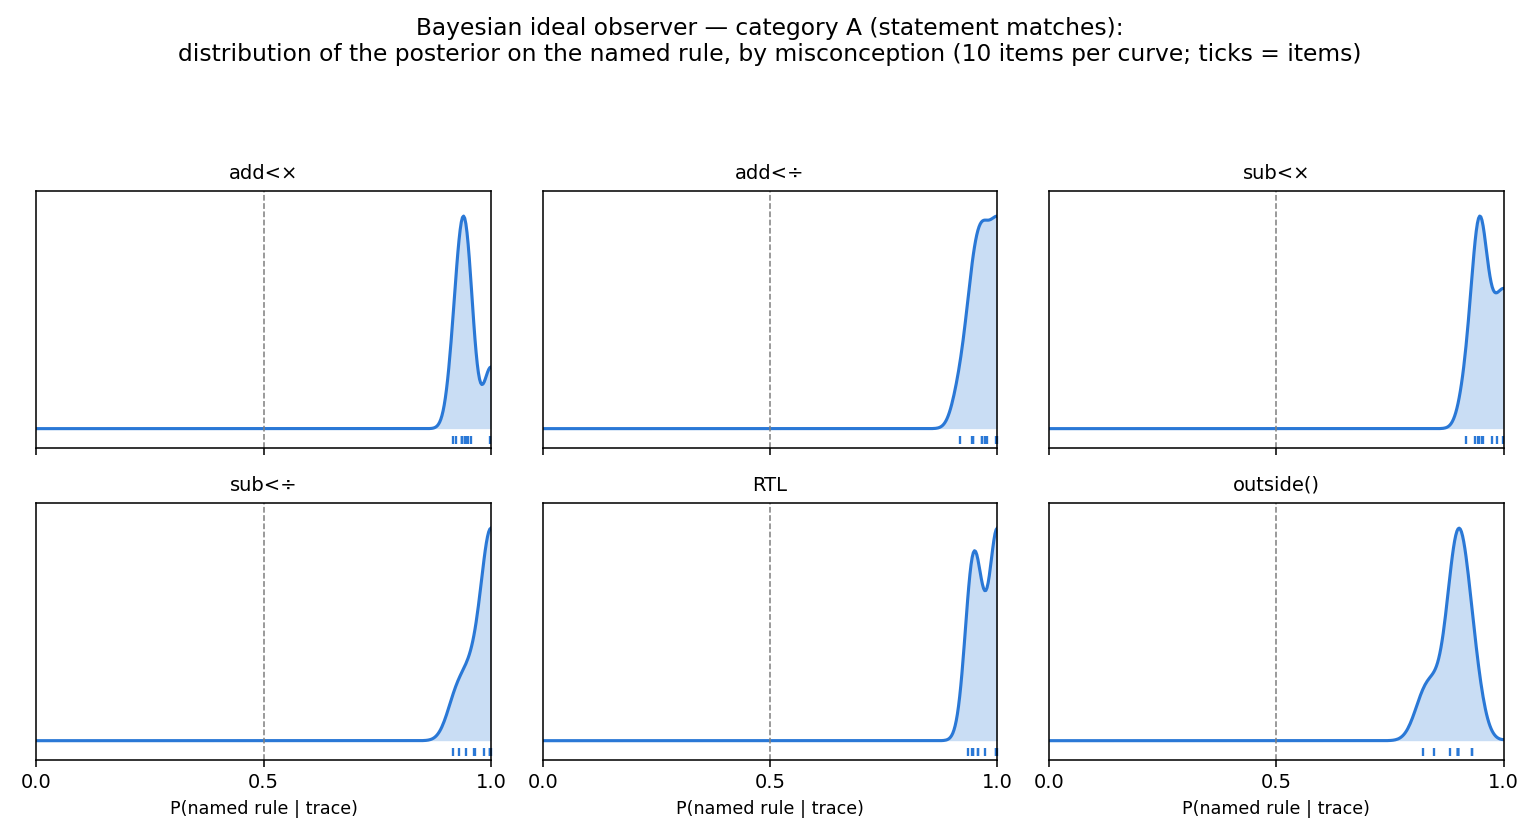
\includegraphics[width=0.85\textwidth]{figs/bayes_1misc_dist_A.png}
\caption{Ideal observer, category A (statement matches the work; agreeing is correct).
Each panel is the distribution of the posterior marginal on the named rule over that
misconception's 10 items (curves are boundary-reflected kernel densities; the ticks underneath
are the individual items). All items sit far right of the 0.5 decision boundary;
\texttt{outside\_bracket\_first} is the one visibly weaker case.}
\label{fig:bayes1a}
\end{figure}

\subsection{Category B: the named misconception is absent}\label{sec:bayes-1misc-b}

Figure~\ref{fig:bayes1b} shows the same quantity for the 60 foil items, in three rows.
Row~1 groups the items by the misconception actually \emph{present} in the trace, asking
whether some student bugs make the work more confusable. Row~2 regroups the same 60 items by
the misconception \emph{named} in the statement, asking whether some claims are easier to rule
out. Row~3 keeps only the \emph{refuted} subset of row~2: items on which the marginal falls
below 0.15 because the trace reached a decision point where a student who truly held the named
rule would have acted differently, and the student visibly acted conventionally instead.

Two regularities stand out. First, every item in rows 1 and 2 sits below the 0.5 boundary
(thresholded accuracy is again 100\%), but the distributions are bimodal: a cluster near
0.17 to 0.26, where the named rule simply never had an opportunity to express itself and the
observer retains a residual possibility that the student holds it silently, and a second
cluster near zero. \sethlcolor{green}\hl{The row~1 panels are nearly interchangeable, so the structure is not driven
by what the student actually did;} \sethlcolor{yellow}\hl{the row~2 panels differ sharply, so it is driven by the
claim itself.} Same-priority (\texttt{RTL}) claims are refutable most often (4 of 10 items),
because equal-priority configurations occur in almost every expression, whereas
\texttt{sub\_before\_div} claims are never refutable in the deployed pool (0 of 10): a
subtraction-next-to-division decision point never arises in those traces. The row~3
\texttt{sub\_before\_div} panel therefore shows one supplementary generated item that fills
this gap; the deployed pool itself contains no such case.

Second, wherever an item is refutable, the distribution shifts sharply left: the refuted
subset in row~3 collapses onto zero (0.00 to 0.03) for every misconception except
\texttt{outside\_bracket\_first}, whose three refuted items settle near 0.12. Bracket
contradictions are soft in the same way that bracket support is weak in
Figure~\ref{fig:bayes1a}. Overall only 12 of the 60 foil items are refutable at all, so for
about 80\% of foils even an ideal reasoner cannot find a contradiction; the correct route to
disagreement is noticing the absence of support, not the presence of counter-evidence.

\begin{figure}[H]
\centering
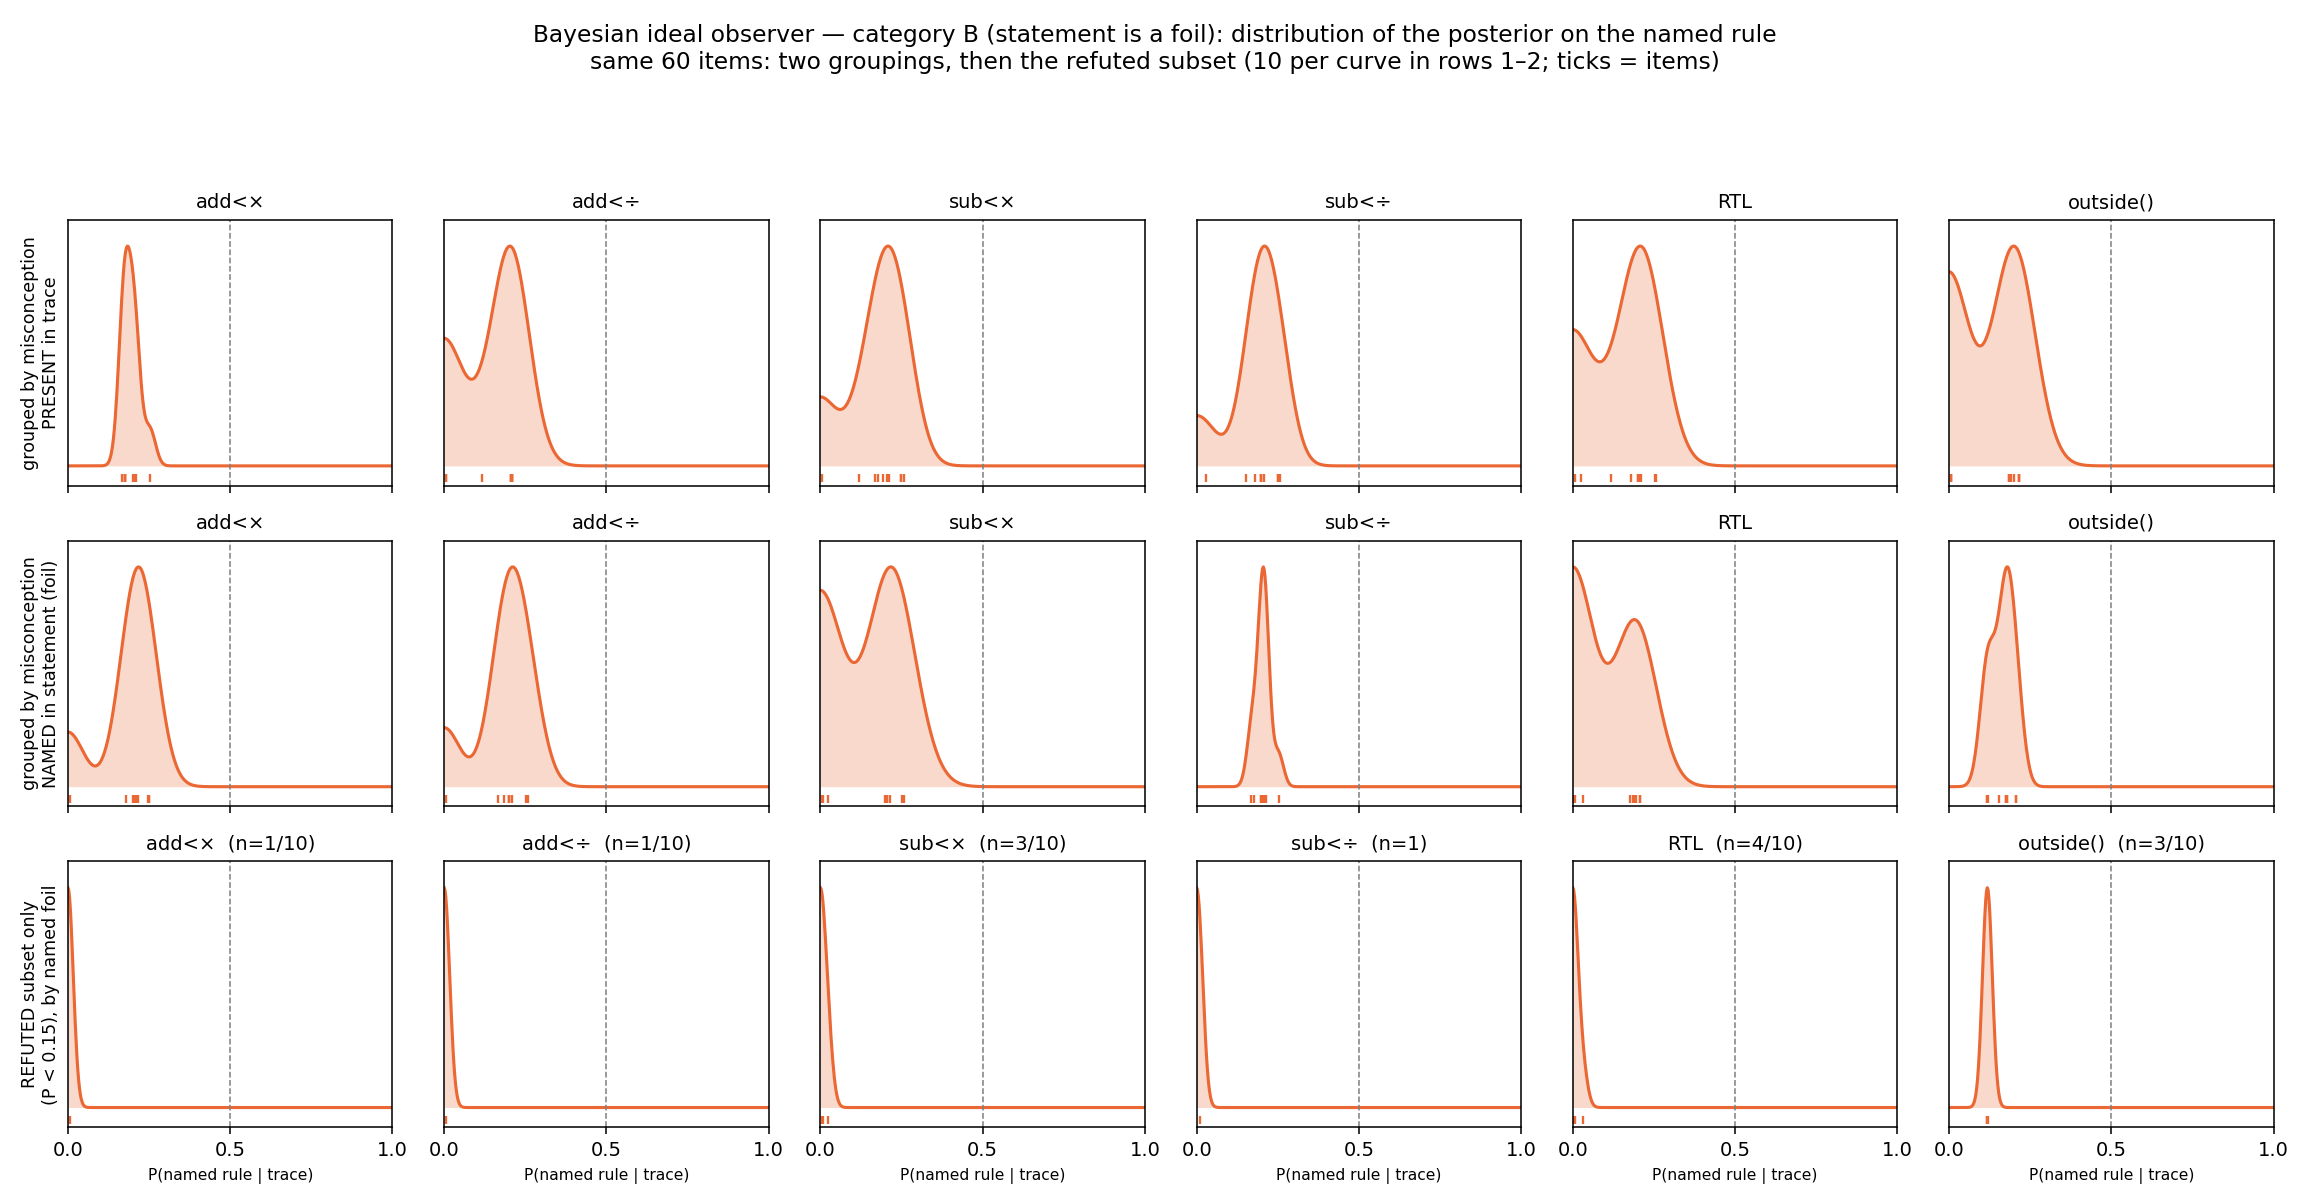
\includegraphics[width=\textwidth]{figs/bayes_1misc_dist_B.png}
\caption{Ideal observer, category B (statement names an absent misconception; disagreeing is
correct). Row 1: the 60 foil items grouped by the misconception present in the trace. Row 2:
the same items grouped by the misconception named in the statement. Row 3: only the refuted
items (marginal below 0.15), grouped as in row 2, with per-panel counts; the
\texttt{sub\_before\_div} panel shows one supplementary generated item because the deployed
pool contains no refutable case for that foil. Rows 1 and 2 are bimodal (unsupported items at
roughly 0.2, refuted items near 0); row 3 isolates the refuted items and the distributions
collapse onto zero, except the softer bracket cases.}
\label{fig:bayes1b}
\end{figure}


%----------------------
\section{LLMs: one-misconception items}\label{sec:llm-1misc}

Three model regimes performed the identical task with the identical instructions, stimuli,
and 1--6 response scale as the human participants: \textbf{haiku (thinking)}
(claude-haiku-4.5 with extended reasoning), \textbf{haiku (direct)} (the same model with
reasoning disabled), and \textbf{gpt-4o (direct)} (gpt-4o ignores the reasoning flag, so it
runs once). Each regime rated every pool item exactly once at temperature 0, so each panel
below rests on 10 deterministic ratings per regime. Curves pass through the exact proportion
of items at each rating (dots); where a curve lies on the axis, that regime literally never
used that rating. The dashed line at 3.5 separates disagreement from agreement.

\subsection{Category A: the named misconception is present}\label{sec:llm-1misc-a}

Figure~\ref{fig:llm1a} shows a three-way split. Haiku (thinking) behaves like a softened
ideal observer: its mass sits at ratings 5 and 6 in every panel (on \texttt{add\_before\_div}
it rates all 10 items exactly 6), and it is the only regime that ever uses the middle of the
scale, doing so mainly for \texttt{same\_priority\_rtl} and \texttt{outside\_bracket\_first},
the same items where the ideal observer's evidence is weakest. The two no-reasoning regimes
are near-binary (their curves lie on zero across ratings 2 to 4) and split the claims between
them in opposite, claim-specific ways. Haiku (direct) endorses most true add/sub statements
(0.5 to 0.8 of items at rating 6) yet flatly rejects true \texttt{RTL} and \texttt{outside()}
statements (0.8 to 0.9 of items at rating 1). Gpt-4o (direct) does the reverse: it rejects
half or more of the true add/sub statements while endorsing \texttt{RTL} and
\texttt{outside()} ones. Neither pattern tracks the strength of the evidence; both track the
identity of the claim.

\begin{figure}[H]
\centering
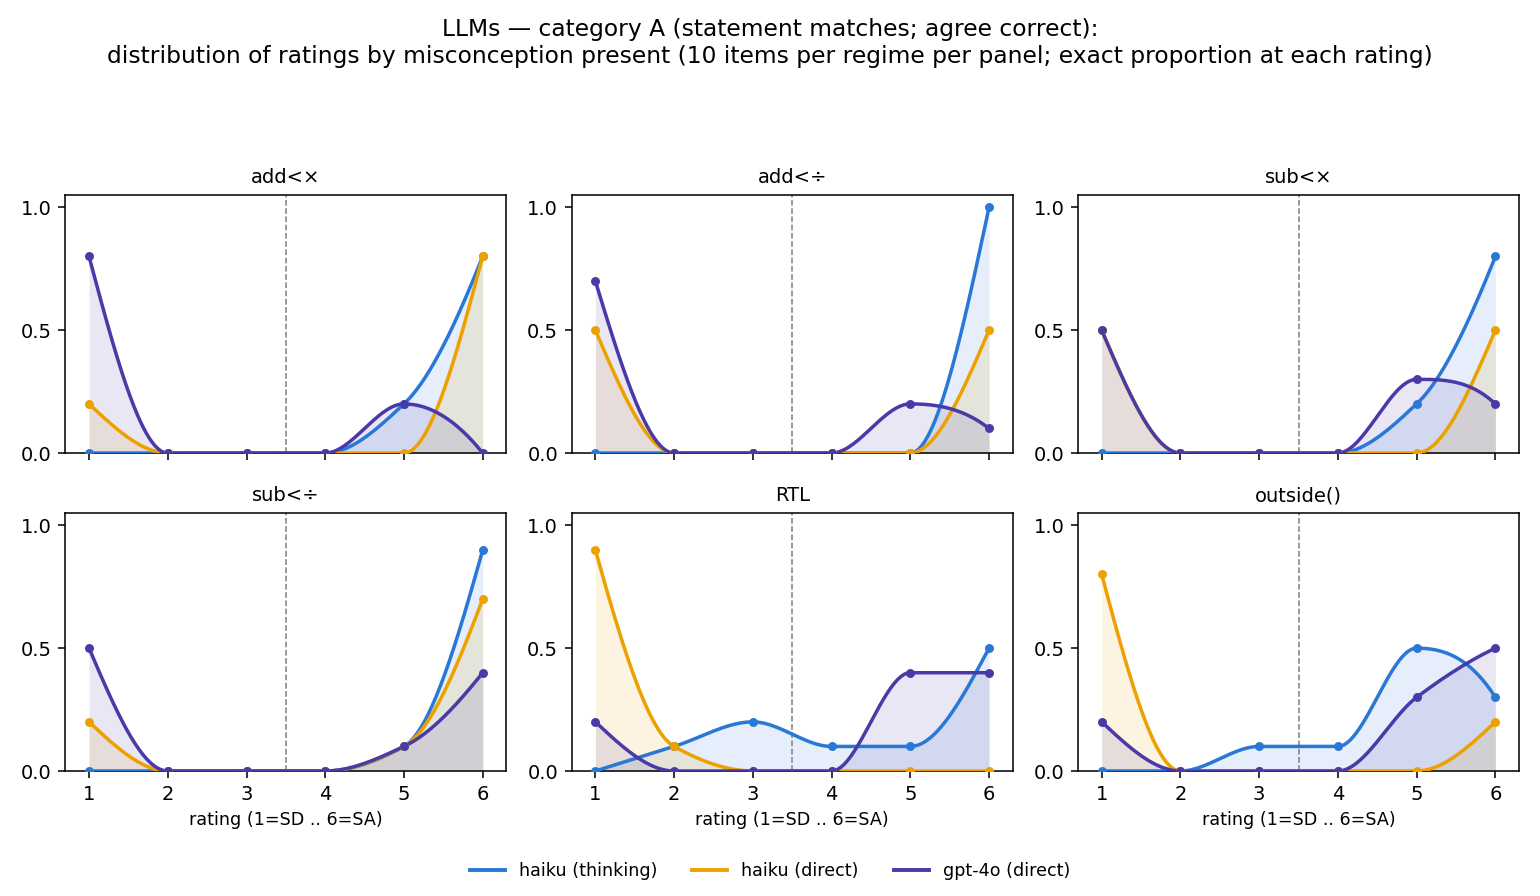
\includegraphics[width=0.95\textwidth]{figs/llm_1misc_dist_A.png}
\caption{LLMs, category A (statement matches the work; agreeing is correct). One curve per
regime; y-axis is the exact proportion of that regime's 10 items at each rating, and dots mark
the exact values. Haiku (thinking) concentrates on 5--6 throughout; the two direct regimes are
near-binary and disagree with each other about \emph{which} claims to endorse.}
\label{fig:llm1a}
\end{figure}

\subsection{Category B: the named misconception is absent}\label{sec:llm-1misc-b}

Figure~\ref{fig:llm1b} uses the same three rows as the ideal-observer figure: foils grouped by
the misconception present, by the misconception named, and the refuted subset only. Haiku
(direct) spikes at rating 1 in essentially every panel of rows 1 and 2: it rejects nearly all
foils, which is correct here but is the same reflexive disagreement it applied to the true
\texttt{RTL} and \texttt{outside()} statements in category A. Haiku (thinking) concentrates on
1 and 2 with a modest graded tail. Gpt-4o again mirrors its category-A signature: it rejects
add/sub foils outright yet endorses a large share of \texttt{RTL} and \texttt{outside()}
foils (for foils naming \texttt{outside\_bracket\_first}, half of its ratings land at 5),
giving false alarms concentrated entirely on the two claims it favors.

The refuted row is where the regimes separate most cleanly. Haiku (thinking) shifts sharply
left, like the ideal observer: on refuted items its ratings collapse onto 1 and 2, so it
demonstrably registers the contradicting step. Gpt-4o does not: it rates the refuted
\texttt{add\_before\_div} item 6 and refuted \texttt{outside()} items 5 to 6, endorsing
claims that the student's own work contradicts. The single \texttt{sub\_before\_div} panel
(the supplementary generated item, whose trace shows the student taking the division first at
a live subtraction-division choice point) makes the contrast explicit: haiku (thinking) rates
it 2, gpt-4o rates it 5, and haiku (direct), which rejects nearly everything else, rates it 6.
Both no-reasoning models read ``the subtraction happened early'' and endorse the claim without
checking which operator the subtraction actually preceded.

\begin{figure}[H]
\centering
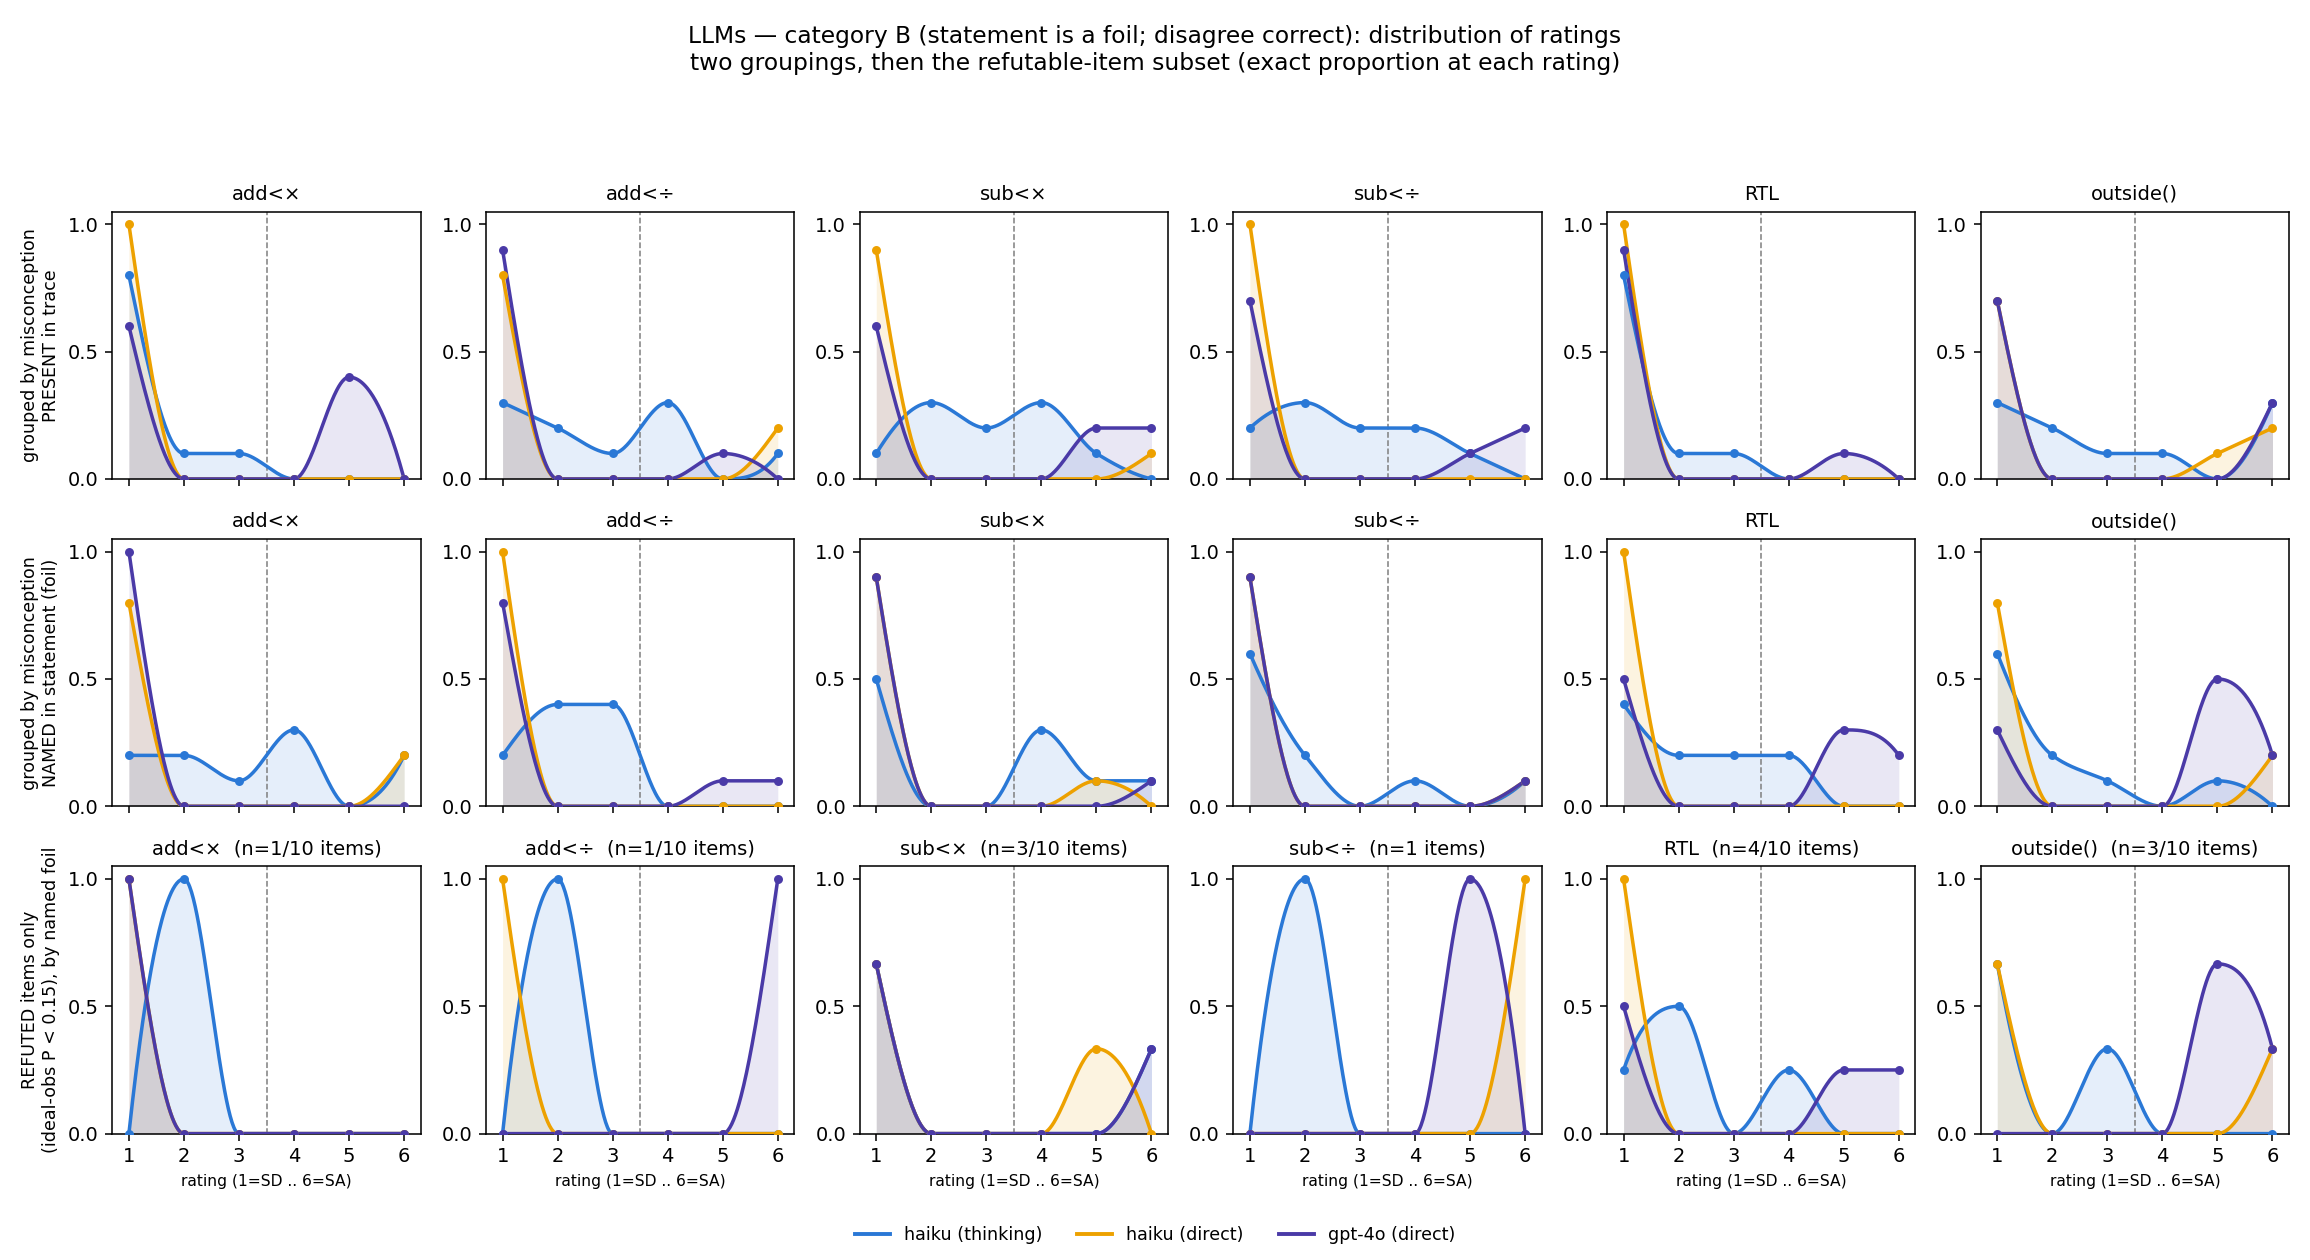
\includegraphics[width=\textwidth]{figs/llm_1misc_dist_B.png}
\caption{LLMs, category B (statement names an absent misconception; disagreeing is correct),
in the same three-row layout as the ideal-observer figure: by misconception present, by
misconception named, and the refuted subset only. Haiku (thinking) shifts left on refuted
items, as the ideal observer does; gpt-4o endorses several claims the work explicitly
contradicts; haiku (direct) rejects everything except the generated
\texttt{sub\_before\_div} item, which it rates 6.}
\label{fig:llm1b}
\end{figure}

%----------------------
\section{Humans: one-misconception items}\label{sec:human-1misc}

Twenty-four Prolific participants each completed 24 trials (6 per category, balanced so that
every misconception appears exactly once as the present misconception in their A trials and
once in their B trials), giving 24 trials per panel below. Ratings are collapsed to a binary
response, the same collapse used for accuracy scoring: 1 to 3 counts as disagree (red) and
4 to 6 as agree (green). Each panel shows the probability of the two responses with raw trial
counts on the bars; the dashed line marks 0.5.

\subsection{Category A: the named misconception is present}\label{sec:human-1misc-a}

Humans were bad at this half of the task. Where the ideal observer endorses every category-A
statement with high confidence and haiku (thinking) concentrates on ratings 5 and 6,
Figure~\ref{fig:human1a} shows humans hovering at a coin flip for every misconception:
$P(\text{agree})$ runs from 0.46 to 0.54 across five of the six panels. The one departure is
in the wrong direction: for \texttt{add\_before\_mul} the majority actively disagrees with a
true statement (9 agree versus 15 disagree, $P(\text{agree}) = 0.38$). Recognizing that a
correctly named misconception explains the work is the part of the task humans could not do
reliably.

\begin{figure}[H]
\centering
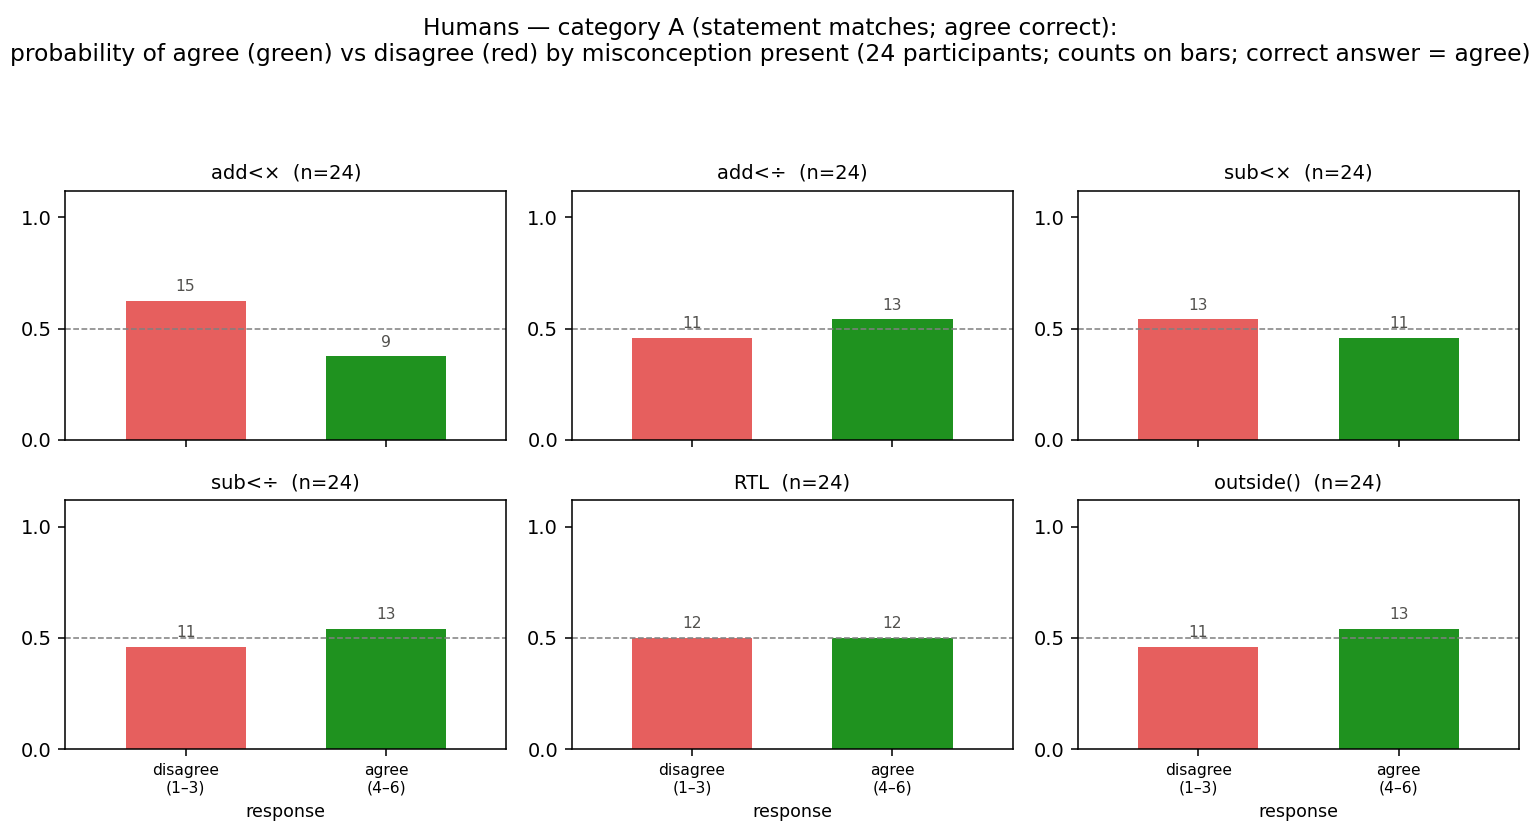
\includegraphics[width=0.85\textwidth]{figs/human_1misc_dist_A.png}
\caption{Humans, category A (statement matches the work; agreeing is correct). Bars are the
probability of each binary response (green = agree, red = disagree), with trial counts on
top. Every misconception sits at or near chance, and \texttt{add\_before\_mul} is below it.}
\label{fig:human1a}
\end{figure}

\subsection{Category B: the named misconception is absent}\label{sec:human-1misc-b}

Figure~\ref{fig:human1b} uses the same three rows as the two previous sections: foils grouped
by the misconception present, by the misconception named, and the refuted subset only. \sethlcolor{green}\hl{Here
humans are better: correct rejection (a taller red bar) is the majority response in almost
every panel.} Exactly two cells in the figure cross the 0.5 line, and they isolate the two
human failure modes. In row~1, traces containing \texttt{outside\_bracket\_first} are the only
case where the majority endorses a false claim ($P(\text{agree}) = 0.58$): work with mangled
brackets looks disordered enough that any accusation becomes believable. In row~2, foils
naming \texttt{add\_before\_div} are the only claim endorsed more often than not (0.54),
typically when the addition in the trace really did fire early but before a different
operator. In the refuted row the false-alarm rate drops relative to row~2 for every foil with
usable data (pooled 0.29 versus 0.39; for \texttt{add\_before\_div} foils, 0.25 versus 0.54),
so participants do exploit an explicit contradiction when the trace contains one. The
\texttt{sub\_before\_div} panel is empty because the deployed pool contains no refutable item
for that foil; the supplementary generated item of the previous sections was never shown to
humans.

\begin{figure}[H]
\centering
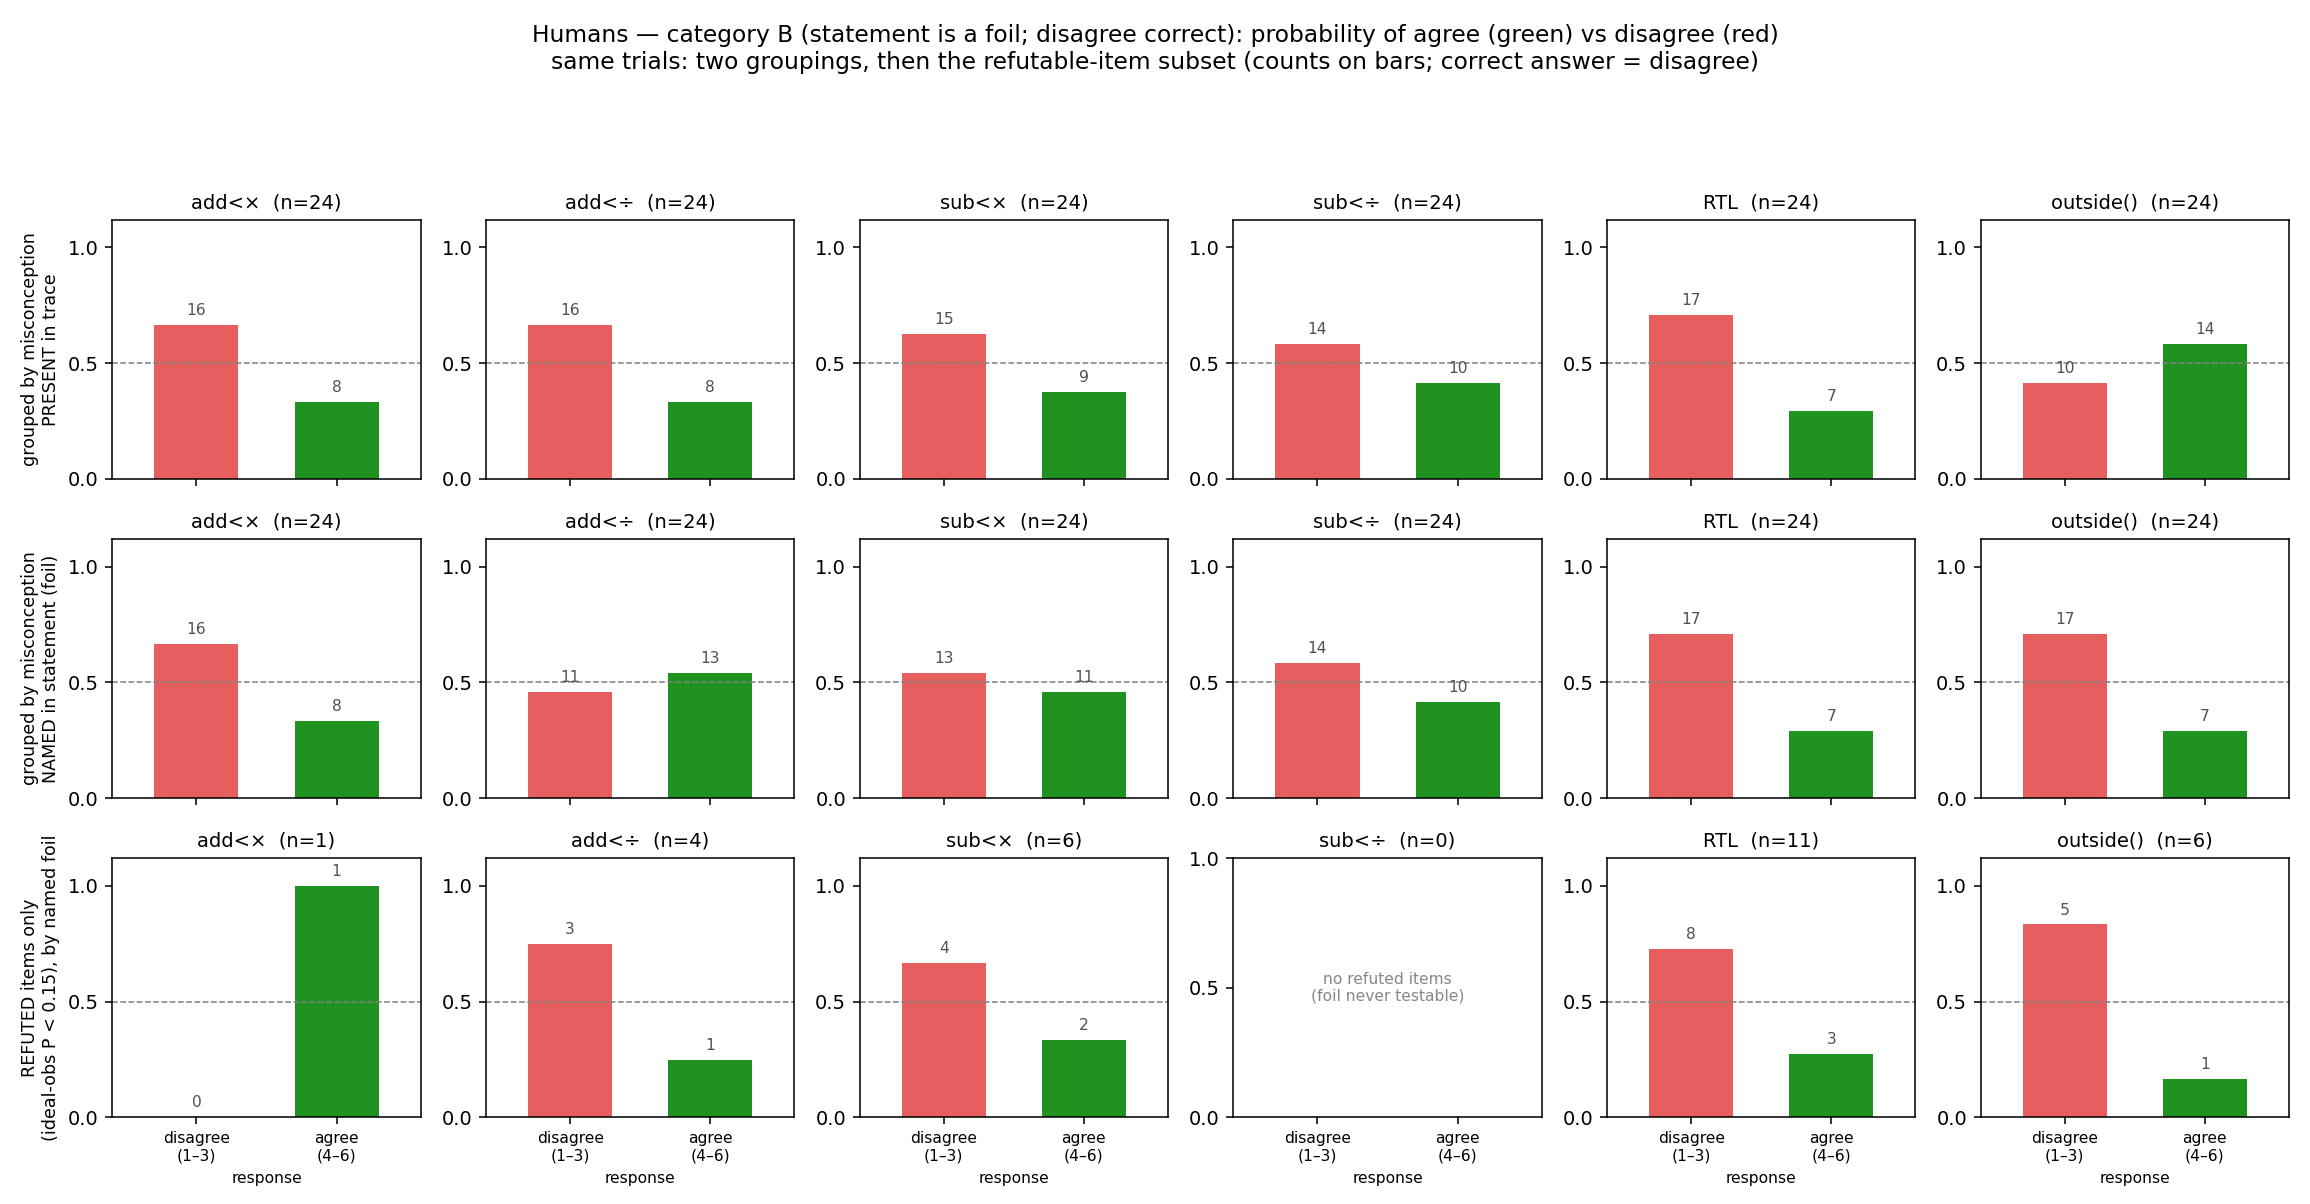
\includegraphics[width=\textwidth]{figs/human_1misc_dist_B.png}
\caption{Humans, category B (statement names an absent misconception; disagreeing is
correct), in the same three-row layout as the ideal-observer and LLM figures. Only two cells
cross 0.5: traces containing bracket errors (row 1) and foils naming
\texttt{add\_before\_div} (row 2). On refutable items (row 3) false alarms drop below the
corresponding row-2 rates.}
\label{fig:human1b}
\end{figure}

\subsection{Individual differences: the average hides two populations}\label{sec:human-1misc-sdt}

The chance-level averages above are not a description of a typical participant. Treating
agree as a yes response (signal = statement true, noise = foil), each participant's hit and
false-alarm rates give a sensitivity $\dpr = z(\text{hit}) - z(\text{FA})$; \sethlcolor{green}\hl{zero means the
participant cannot distinguish true statements from foils at all.} Figure~\ref{fig:humansdt}
shows the result: pooled over everyone, sensitivity is weak ($\dpr = 0.51$) with a nearly
neutral criterion, but the per-participant values span $-1.64$ to $+2.77$. \sethlcolor{green}\hl{Three participants
reach $\dpr \geq 2$, and the best (92\% accuracy, $\dpr = 2.77$) outperforms every LLM regime
on the identical pool.} \sethlcolor{yellow}\hl{At the other end, about seven participants sit at chance and two are
reliably below it: one answered disagree on 23 of 24 trials, and one spent 11 minutes
answering systematically opposite to the key, a pattern consistent with misreading the scale
or the question rather than low effort (response times showed no participant answering faster
than 4 seconds per trial).} A substantial share of the sample either never understood the task
or adopted a degenerate strategy, which is why we are considering adding practice trials with
feedback (the current experiment gates entry with a single comprehension question and no
practice) before the confirmatory run.

\begin{figure}[H]
\centering
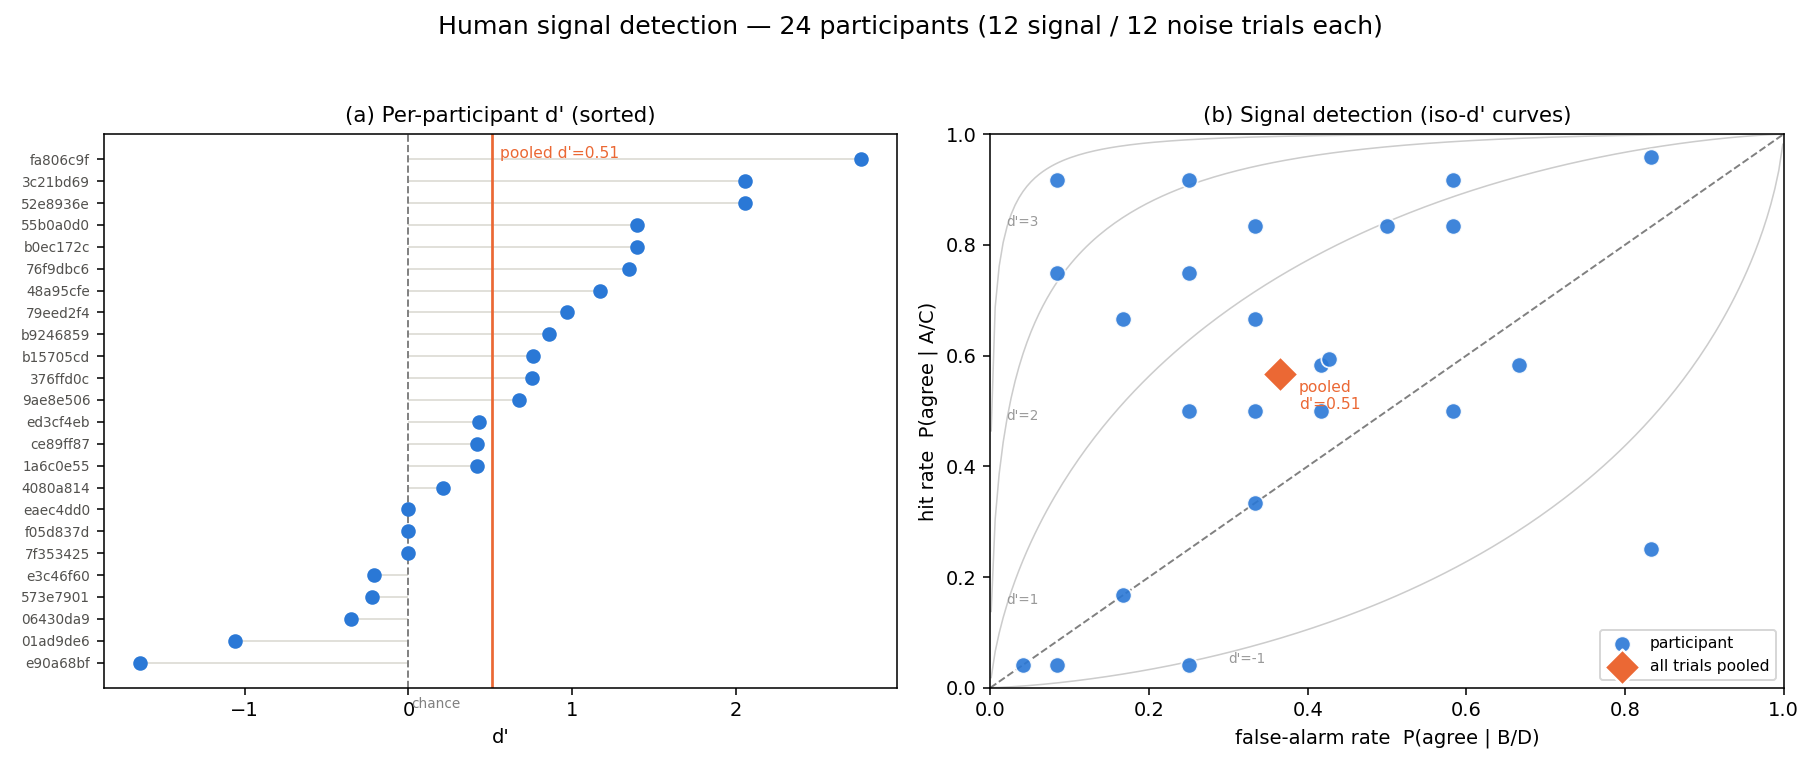
\includegraphics[width=\textwidth]{figs/human_signal_detection.png}
\caption{Human signal detection over all 24 trials per participant (12 statement-true, 12
foil). Left: per-participant $\dpr$, sorted; the orange line is the pooled value. Right: each
participant in ROC space (hit rate versus false-alarm rate) against iso-$\dpr$ curves; the
diamond is the pooled point, and points below the diagonal are participants who answered
systematically opposite to the key. The spread from $-1.64$ to $+2.77$, rather than the weak
pooled value, is the central human result.}
\label{fig:humansdt}
\end{figure}

%----------------------
\section{Two-misconception items: present $\times$ shown heatmaps}\label{sec:2misc}

The remaining 120 items contain \emph{two} misconceptions in the trace. In category C the
statement names one of the two (a true but partial explanation; agreeing is correct), and in
category D it names neither (a foil; disagreeing is correct). Because a response now depends
on two things at once, what pair is present in the work and what the statement claims, we
summarize these items as present $\times$ shown heatmaps. The same two-panel design is used
for all three observers, so it is described once here.

Panel (a) covers category C as a $6 \times 6$ square: the row is the misconception NAMED in
the statement (the probed target, which is genuinely present), the column is the OTHER
misconception present alongside it, so each cell is one target-partner combination and the
diagonal is impossible (a learner cannot hold the same misconception twice). Panel (b) covers
category D as a $6 \times 15$ rectangle: the row is the named foil (absent from the work), the
column is the PAIR actually present. Within a foil's row only the 10 pairs that do not contain
the foil are possible; the impossible cells are gray. Cells are colored on a diverging scale,
green toward the agree side and red toward the disagree side, so a correct observer shows a
green panel (a) and a red panel (b). For humans and LLMs the cell value is the mean 1--6
rating, centered at 3.5; for the ideal observer it is the mean posterior marginal on the named
rule, centered at 0.5. Each cell is annotated with its value and the number of observations it
rests on.

\subsection{Bayesian ideal observer}\label{sec:bayes-2misc}

Figure~\ref{fig:bayes2} shows that the two-misconception items remain unambiguous for an
observer that actually inverts the generative model. In panel (a) every cell is green: the
mean marginal on the named target ranges from 0.76 to 1.00, so no partner misconception ever
masks a genuinely present target enough to matter. The two weakest cells both have
\texttt{outside\_bracket\_first} as the named target (0.76 with a \texttt{sub\_before\_mul}
partner, 0.80 with an \texttt{RTL} partner), the same bracket weakness that ran through the
one-misconception results. In panel (b) every cell is red and nearly uniform: the marginal on
the named foil never exceeds 0.26, whichever pair is actually present. The ideal observer has
no confusion structure here; whatever confusions appear in the human and LLM versions of this
figure are properties of those observers, not information missing from the stimuli. (Cell
counts are small by design: panel (a) cells hold 1 to 4 items and panel (b) exactly one item
per foil-pair combination, but the observer is deterministic, so these are exact item-level
values rather than noisy samples.)

\begin{figure}[H]
\centering
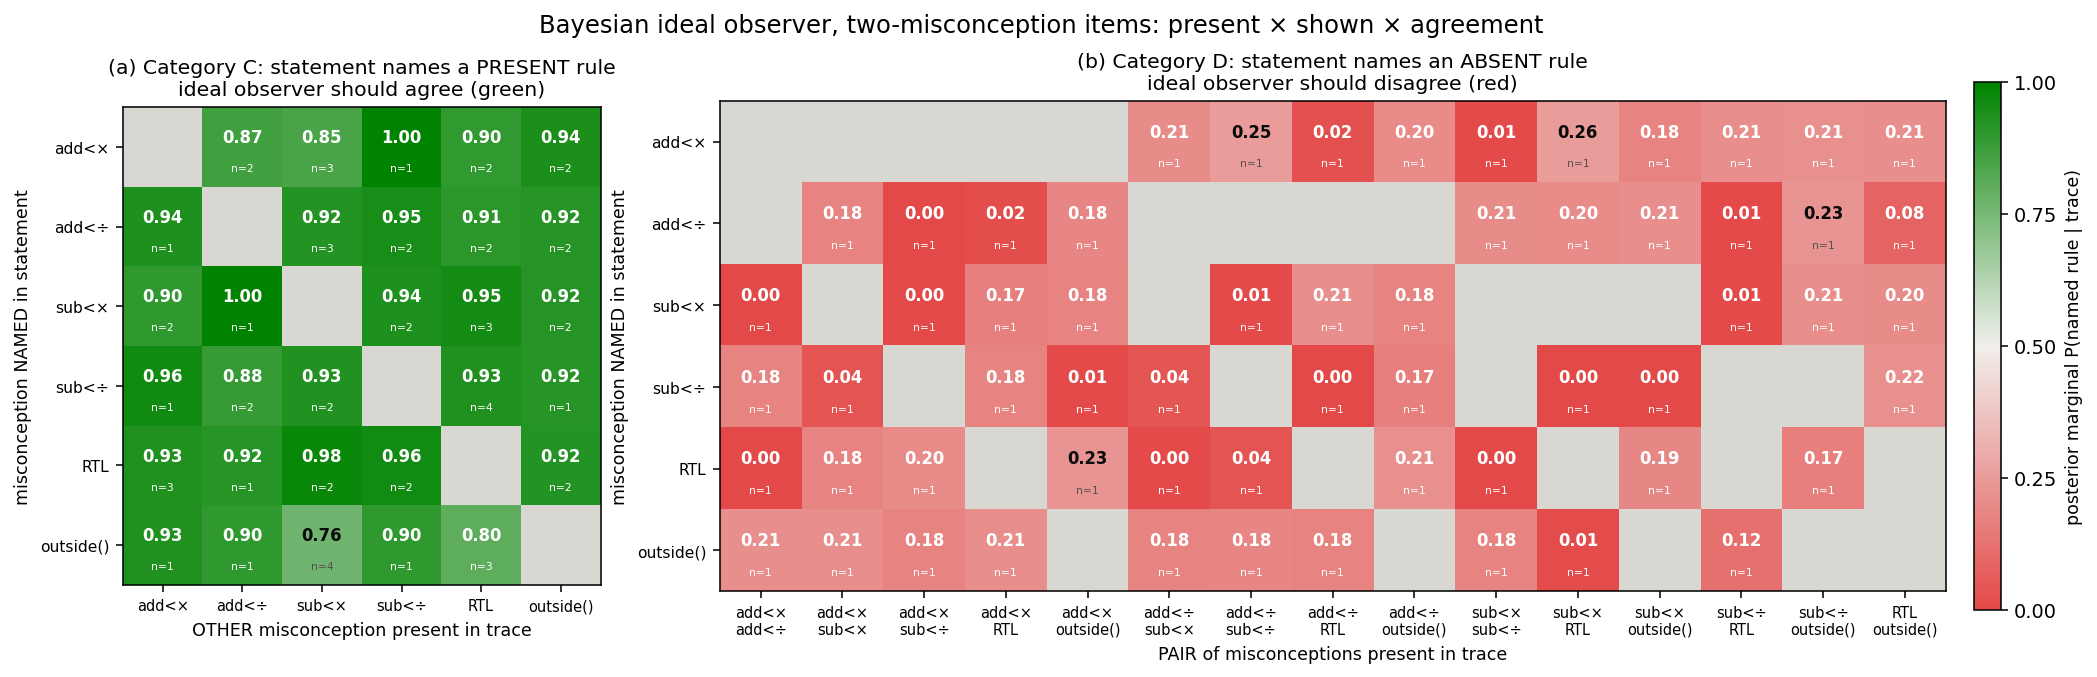
\includegraphics[width=\textwidth]{figs/bayes_2misc_heatmap.png}
\caption{Ideal observer, two-misconception items. Panel (a), category C: mean marginal on the
named target (present), rows, by the other misconception present, columns; agreeing is
correct, so green throughout is ideal. Panel (b), category D: mean marginal on the named foil
(absent), rows, by the pair actually present, columns; disagreeing is correct, so red
throughout is ideal. Gray cells are structurally impossible. The observer is near ceiling in
both panels; its only soft spots are bracket claims as the named target in panel (a).}
\label{fig:bayes2}
\end{figure}

\subsection{LLMs}\label{sec:llm-2misc}

Figure~\ref{fig:llm2} repeats the two panels for each regime (one row per regime). As with the
ideal observer, the cell values are exact rather than sampled: each regime rated every item
once at temperature 0, so a panel (a) cell averages 1 to 4 deterministic ratings and every
panel (b) cell is the single rating of its one item.

\sethlcolor{yellow}\hl{Haiku (thinking) again approximates the ideal observer. Its panel (a) is green nearly
throughout:} partial explanations are endorsed for almost every target-partner combination,
with its few tepid cells involving \texttt{RTL} as target or partner. \sethlcolor{yellow}\hl{Its panel (b) is mostly
red, but the false alarms it does make are systematic rather than scattered: the
\texttt{add\_before\_mul} foil row lights up on pairs that contain
\texttt{add\_before\_div} (ratings up to 6), the same operation-family confusion that
appeared in its one-misconception results.} The claim ``the addition happened too early'' is
accepted when addition did fire early, without verifying which operator it preceded.

The two no-reasoning regimes reproduce their category-A/B signatures. Haiku (direct) turns
panel (b) into a wall of 1s, rejecting every foil, but pays for it in panel (a), which is
largely red: it also rejects most of the true partial explanations (its \texttt{RTL}-target
row is uniformly 1.0). Its correct panel (b) is the by-product of a blanket disagree policy,
not of reading the work. Gpt-4o (direct) is claim-driven in both panels at once: its
\texttt{RTL} and \texttt{outside()} rows are green in panel (a) \emph{and} in panel (b),
meaning it endorses those two claims whether they are true of the work or not (false alarms
up to 6 across several different pairs), while add/sub claims are mostly rejected in both
panels regardless of the evidence. Since the ideal observer's panel (b) is flat and low on
identical items, all of this structure belongs to the observers, not the stimuli.

\begin{figure}[H]
\centering
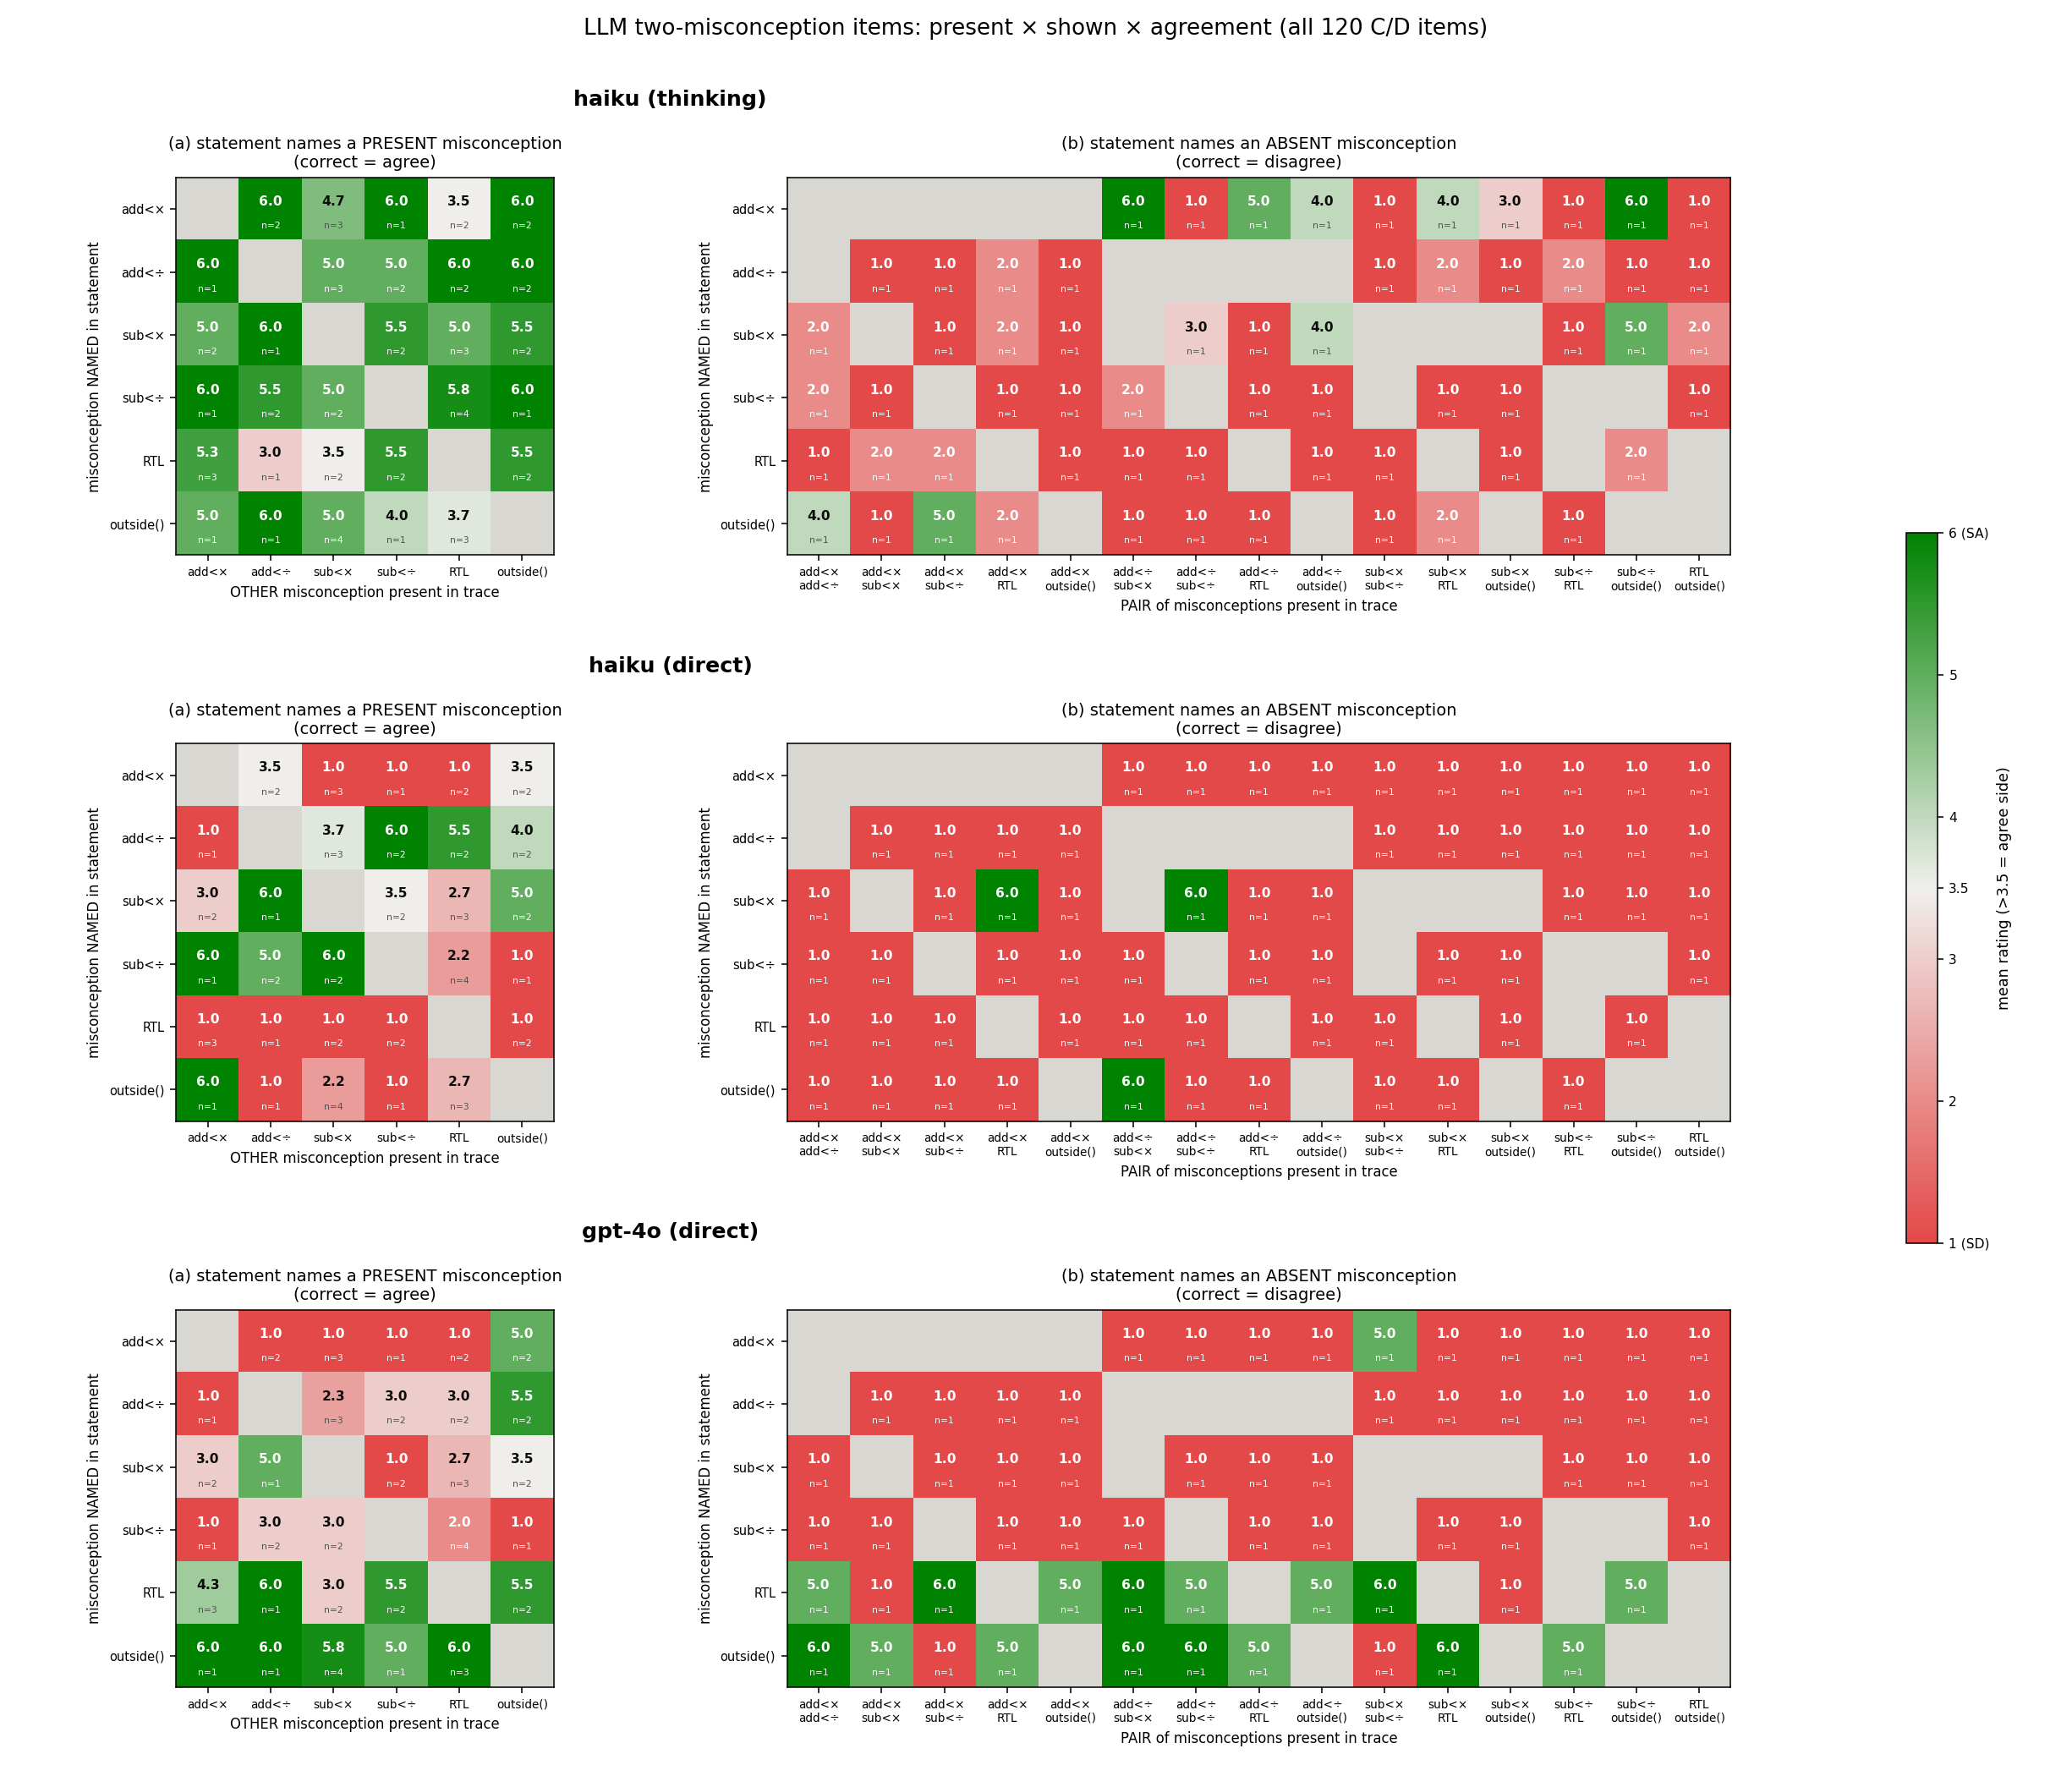
\includegraphics[width=\textwidth]{figs/llm_2misc_heatmap.png}
\caption{LLMs, two-misconception items, one row of panels per regime (same layout and color
scale as Figure~\ref{fig:bayes2}). Haiku (thinking): green panel (a), red panel (b) except
for operation-family confusions concentrated in the \texttt{add\_before\_mul} foil row.
Haiku (direct): rejects nearly everything in both panels, so it is right on foils for the
wrong reason. Gpt-4o (direct): endorses \texttt{RTL} and \texttt{outside()} claims in both
panels regardless of what the trace shows.}
\label{fig:llm2}
\end{figure}


\subsection{Humans}\label{sec:human-2misc}

Figure~\ref{fig:human2} shows the human version. Unlike the two previous figures these cells
are noisy behavioral averages: the 24 participants contribute 144 category-C and 144
category-D trials, so panel (a) cells hold 1 to 11 trials, panel (b) cells 0 to 6, and a dot
marks a foil-pair combination that no participant happened to draw. The patterns below should
therefore be read as exploratory structure.

In panel (a) humans sit in the middle of the scale rather than at the green ceiling, and the
structure runs along both axes. By row, naming a subtraction rule is under-endorsed even
though the claim is true: the \texttt{sub\_before\_mul} and \texttt{sub\_before\_div} rows
average on the disagree side of 3.5, while the \texttt{add\_before\_mul}, \texttt{RTL}, and
\texttt{outside()} rows land on the agree side. By column, the partner matters, which it never
does for the ideal observer: having \texttt{sub\_before\_mul} or \texttt{outside()} as the
\emph{other} misconception in the trace drags endorsement of the named one down (the worst
cell, a true \texttt{sub\_before\_div} statement next to a \texttt{sub\_before\_mul} partner,
averages 1.7). A messy companion error can mask a genuinely present target.

Panel (b) shows where human false alarms live, and their organization is the mirror image of
gpt-4o's. The \texttt{outside()} foil row is uniformly red (no cell above 3.0): a bracket
claim is easy to check against the work and reject. Instead, the strongest false alarms sit in
\emph{columns} whose pair contains \texttt{outside()}: a false \texttt{add\_before\_mul} claim
on an \texttt{add\_before\_div}+\texttt{outside()} trace averages 5.0, false \texttt{RTL} on
\texttt{sub\_before\_mul}+\texttt{outside()} 5.0, false \texttt{sub\_before\_div} on
\texttt{RTL}+\texttt{outside()} 4.7. Work containing mangled brackets looks disordered enough
that unrelated accusations become believable. Humans also share the add-family leak seen in
haiku (thinking): a false \texttt{add\_before\_mul} claim is endorsed when
\texttt{add\_before\_div} is actually present. \sethlcolor{green}\hl{In short, human confusions organize around what
the \emph{trace} looks like, gpt-4o's around what the \emph{claim} says, haiku (thinking)
shares the human operation-family confusion, and the ideal observer, flat on the same items,
shows that none of these confusions is forced by the stimuli.}

\begin{figure}[H]
\centering
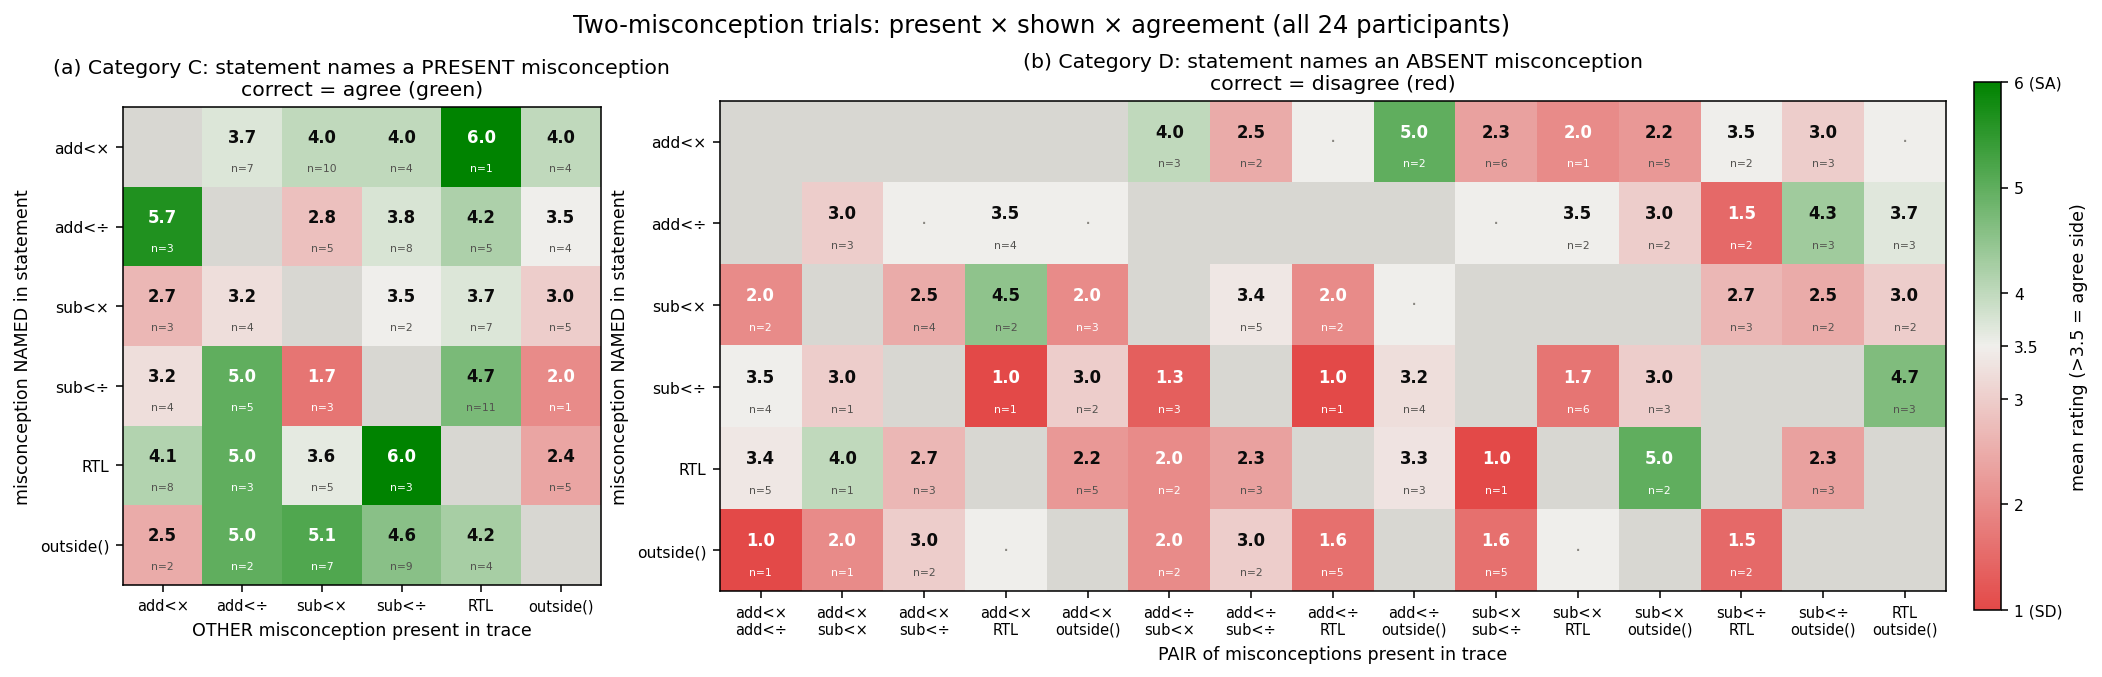
\includegraphics[width=\textwidth]{figs/human_2misc_heatmap.png}
\caption{Humans, two-misconception items (same layout and color scale as
Figure~\ref{fig:bayes2}; cell values are mean ratings over the trials in the cell, dots mark
combinations no participant drew). Panel (a): true partial explanations are endorsed only
weakly, subtraction rules least, and a \texttt{sub\_before\_mul} or \texttt{outside()}
partner masks the named target. Panel (b): bracket foils are reliably rejected (bottom row
red), while the strongest false alarms occur when the pair present in the trace contains
\texttt{outside()}, i.e.\ when the work itself looks mangled.}
\label{fig:human2}
\end{figure}
\end{document}
